\documentclass[a4paper]{article}
\usepackage{a4wide}
\usepackage{tikz}


\pagestyle{empty}

\begin{document}

\section{Inleiding}
Deze opgave kan zowel in Java als JavaScript gemaakt worden.
Vermoedelijk zal je het eenvoudiger vinden om het eerst in Java te maken,
gezien deze structurele elementen aanbiedt (klassen). In JavaScript
zal je dezelfde structuur moeten faken d.m.v.\ arrays (bv. de klasse Vak
die twee velden heeft in Java zal een array van 2 elementen zijn in JavaScript,
waarbij het eerste de naam bevat en het tweede de punten).

\section{Beschrijving van de datastructuur}
\begin{itemize}
  \item Een \emph{klas} bestaat uit een aantal studenten. Een klas heeft een bepaalde capaciteit, m.a.w.\ kan
        een maximaal aantal studenten bevatten.
  \item Een \emph{student} heeft een naam en volgt nul of meer vakken.
  \item Een \emph{vak} heeft een naam en een gehaalde score op 20.
\end{itemize}

\begin{center}
  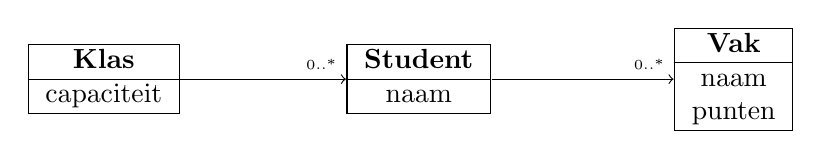
\begin{tikzpicture}
    \node[inner sep=0mm] (klas) at (0,0) { \begin{tabular}{|c|} \hline {\bf Klas} \\ \hline capaciteit \\ \hline \end{tabular} };
    \node[inner sep=0mm] (student) at (4,0) { \begin{tabular}{|c|} \hline {\bf Student} \\ \hline naam \\ \hline \end{tabular} };
    \node[inner sep=0mm] (vak) at (8,0) { \begin{tabular}{|c|} \hline {\bf Vak} \\ \hline naam \\ punten \\ \hline \end{tabular}};

    \draw[->] (klas.east) -- (student.west);
    \draw[->] (student.east) -- (vak.west);

    \node[anchor=south east] at (student.west) { \tiny 0..* };
    \node[anchor=south east] at (vak.west) { \tiny 0..* };
  \end{tikzpicture}
\end{center}

\section{Functionaliteit}
\begin{itemize}
  \item Toevoegen van een nieuwe student aan een klas.
  \item Toevoegen van een nieuw vak aan een student.
  \item Opvragen totaal aantal punten van een student op 100.
  \item Opvragen klasgemiddelde van een bepaald vak op 20.
\end{itemize}

{
\newcommand{\student}[2]{
  \node[inner sep=0mm] (#1) at (#2) { \begin{tabular}{|c|} \hline {\bf :Student} \\ \hline naam:#1 \\ \hline \end{tabular} };
}
\newcommand{\vak}[4][]{
   \node[inner sep=0mm] (#1 #2) at (#4) { \begin{tabular}{|c|} \hline {\bf :Vak} \\ \hline naam:#2 \\ punten:#3 \\ \hline \end{tabular}};
}
\newcommand{\inklas}[1]{
  \draw[->] (klas) -- (#1);
}
\newcommand{\volgt}[2]{
  \draw[->] (#1) -- (#1 #2);
}

\section{Voorbeeld}
We kunnen volgende situatie opbouwen:
\begin{center}
  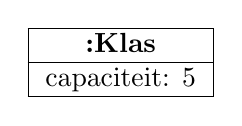
\begin{tikzpicture}
    \node[inner sep=0mm] (klas) at (0,0) { \begin{tabular}{|c|} \hline {\bf :Klas} \\ \hline capaciteit: 5 \\ \hline \end{tabular} };
    \student{Jan}{4,0} \inklas{Jan}
    \student{Piet}{4,1.2} \inklas{Piet}
    \student{Jef}{4,-1.2} \inklas{Jef}

    \vak[Jan]{Algo1}{15}{8,-.75}
    \vak[Jan]{BOP}{13}{8,0.75}
    \volgt{Jan}{Algo1}
    \volgt{Jan}{BOP}

    \vak[Piet]{Algo1}{14}{2.5,3}
    \vak[Piet]{BOP}{16}{5,3}
    \vak[Piet]{Frans}{18}{7.5,3}
    \volgt{Piet}{Algo1}
    \volgt{Piet}{BOP}
    \volgt{Piet}{Frans}

    \vak[Jef]{BOP}{20}{5,-2.75}
    \volgt{Jef}{BOP}
  \end{tikzpicture}
\end{center}
}
\begin{itemize}
  \item Jan heeft als totaal 70, Piet 80 en Jef 100.
  \item Klasgemiddelde voor BOP is 16.3, voor Algo1 14.5 en voor Frans 18.
\end{itemize}


\end{document}